\documentclass[11pt]{article}
\usepackage[margin=1in]{geometry}
\usepackage{amsmath,amssymb,amsthm}
\usepackage{graphicx}
\usepackage[colorlinks=true,linkcolor=blue,citecolor=blue,urlcolor=blue]{hyperref}
\newtheorem{theorem}{Theorem}
\newtheorem{lemma}{Lemma}

\title{The Blades Never Touch the Shore:\ a Proof for the Second Knife of Closed-String Gravity}
\author{Andrei Pluzhnik\thanks{ORCID 0009-0005-5660-2603. Code and data
released with this preprint; companion works: DOI 10.5281/zenodo.21944818
(the shore), DOI 10.5281/zenodo.21947272 (the master formula).}}
\date{August 2026}

\begin{document}
\maketitle

\begin{abstract}
For the graviton family of Cheung, Hillman and Remmen we prove that the
$j{=}3$ trajectory constraint --- the ``second knife'', whose negativity
windows are the blades of our master-formula paper --- never cuts into the
region allowed by the near-leading envelope $\min_k T_k(\lambda)$: for every
level $n$ and every $\lambda>0$, the window of $a_{n,2n-6}$, when it exists,
lies strictly above the shore. The proof is a family of several hundred
positive-coefficient certificates in exact arithmetic: explicit envelope
branches for $\lambda\le26$, and four lemmas for the deep-water tail ---
including the fact that makes the theorem delicate and true at once: the
asymptotic cone of the blades is \emph{exactly tangent} to the shore
asymptote $D=(12+4\sqrt3)\lambda$ (the tangency discriminant vanishes
identically at slope ratio $\rho=1+1/\sqrt3$), while windows only exist up to
$\rho=\sqrt{5/3}$, strictly inside. The closest approach in all of parameter
space is $2.17$ dimensions, at $\lambda\approx0.05$. This upgrades the
$j{=}3$ sector of our completeness conjecture from a $3$-million-point
battery to a theorem.
\end{abstract}

\section{Setup and statement}
Notation as in \cite{master}: $m=n-3$, $s=\lambda+n-1$, $u=D+4m+1$; the
$j{=}3$ rung of the master formula is
$\widehat B_n(u)=\alpha_m\,u(u-2)-G_m\,u\,s^2+s^4$ with
$G_m=\tfrac{2(m+1)(m+3)}{3(2m+3)}$,
$\alpha_m=\tfrac{(m+3)(5m^3+21m^2+19m+15)}{45(2m+1)(2m+3)}$, and
$\operatorname{sign}a_{n,2n-6}=\operatorname{sign}\widehat B_n$. The shore is
$\widehat T(\lambda)=\min_{k\ge3}T_k(\lambda)$ with $T_k$ the trajectory law
of \cite{shore}.

\begin{theorem}[The blades never touch the shore]\label{thm:blades}
For every $n\ge4$ and every $\lambda>0$: if $\widehat B_n(\cdot)$ has a
negativity window in $D$, then its lower edge exceeds
$\widehat T(\lambda)$. Consequently $a_{n,2n-6}\ge0$ everywhere in the
region $D\le\widehat T(\lambda)$.
\end{theorem}

\section{Proof architecture}
All steps are checked in exact rational arithmetic (or exactly over
$\mathbb{Q}(\sqrt3)$); every certificate is a polynomial with manifestly
nonnegative coefficients after an affine--rational change of variables, and
the entire proof re-runs from one script released with this paper.

\textbf{Shallow water ($\lambda\le26.1$): envelope branches.} Fix an integer
$k$ and use $\widehat T\le T_k$: it suffices that on the branch's
$\lambda$-interval every level satisfies \emph{either} no-window
(the discriminant of $\widehat B_n$ is negative --- univariate root
isolation) \emph{or} both $\widehat B_n(T_k)>0$ and the vertex condition
$G_ms^2>(T_k+4m)\,2\alpha_m$ (which together place $T_k$ strictly left of
the window). Branches $k=3,\dots,45$ with rational breakpoints cover
$(0,\,26.1]$; small $m$ are handled per-level (univariately), the $m$-tail
by positive-coefficient certificates. The zone of closest approach
($2.17$ dimensions at $\lambda=0.05$, level $6$) lies in the $k{=}3$ branch,
where the certificates are one substitution deep.

\textbf{Deep water ($\lambda\ge26$): four lemmas.}
\begin{lemma}[No shallow levels]\label{lem:T0}
For $m\le78$ and $\lambda\ge26$ no window exists.
\end{lemma}
\begin{lemma}[Window containment]\label{lem:L2}
For $m\ge79$, windows require $s\le\tfrac43(m+3)$: the discriminant
threshold satisfies
$S^2_{\max}=2\alpha_m\bigl(G_m+2\sqrt{\alpha_m}\bigr)/\beta_m
\le\tfrac{16}{9}(m+3)^2$, $\beta_m=4\alpha_m-G_m^2>0$.
\end{lemma}
\begin{lemma}[Shore below the asymptote]\label{lem:L1}
For $\lambda\ge26$, $\widehat T(\lambda)\le(12+4\sqrt3)\lambda$
(witnessed by $k=\lfloor\sqrt3\lambda\rfloor+2$).
\end{lemma}
\begin{lemma}[Asymptote below the blades]\label{lem:L3}
For $m\ge79$ and $26\le\lambda$ with $s\le\tfrac43(m+3)$, the point
$u_A=(12+4\sqrt3)\lambda+4m+1$ satisfies $\widehat B_n(u_A)>0$ and lies
left of the vertex; hence $u_A$ is strictly left of any window.
\end{lemma}
Chaining Lemmas~\ref{lem:T0}--\ref{lem:L3}: at $\lambda\ge26$ any window
has $m\ge79$ and $s\le\tfrac43(m+3)$, and its lower edge exceeds $u_A$,
which exceeds $u(\widehat T)$. $\qed$

\textbf{The exact tangency.} Why is the deep-water step delicate? In the
scaling limit $m\to\infty$ with $\rho=s/m$ fixed, the window's lower edge and
the shore asymptote compare through the quadratic
$6\rho^2-(12+4\sqrt3)\rho+(8+4\sqrt3)$, whose discriminant is
\emph{identically zero}: the blade cone is exactly tangent to the shore
asymptote, at $\rho^*=1+1/\sqrt3$. The theorem survives because windows only
exist for $\rho\le\sqrt{5/3}<\rho^*$ (Lemma~\ref{lem:L2}): the fleet sails
parallel to the shore, tangent to it at infinity, but its ships are
confined strictly inside the wake. A naive global certificate must fail
(the margin degenerates along $\rho^*$); the containment lemma is what
makes the proof possible.

\begin{figure}[t]
\centering
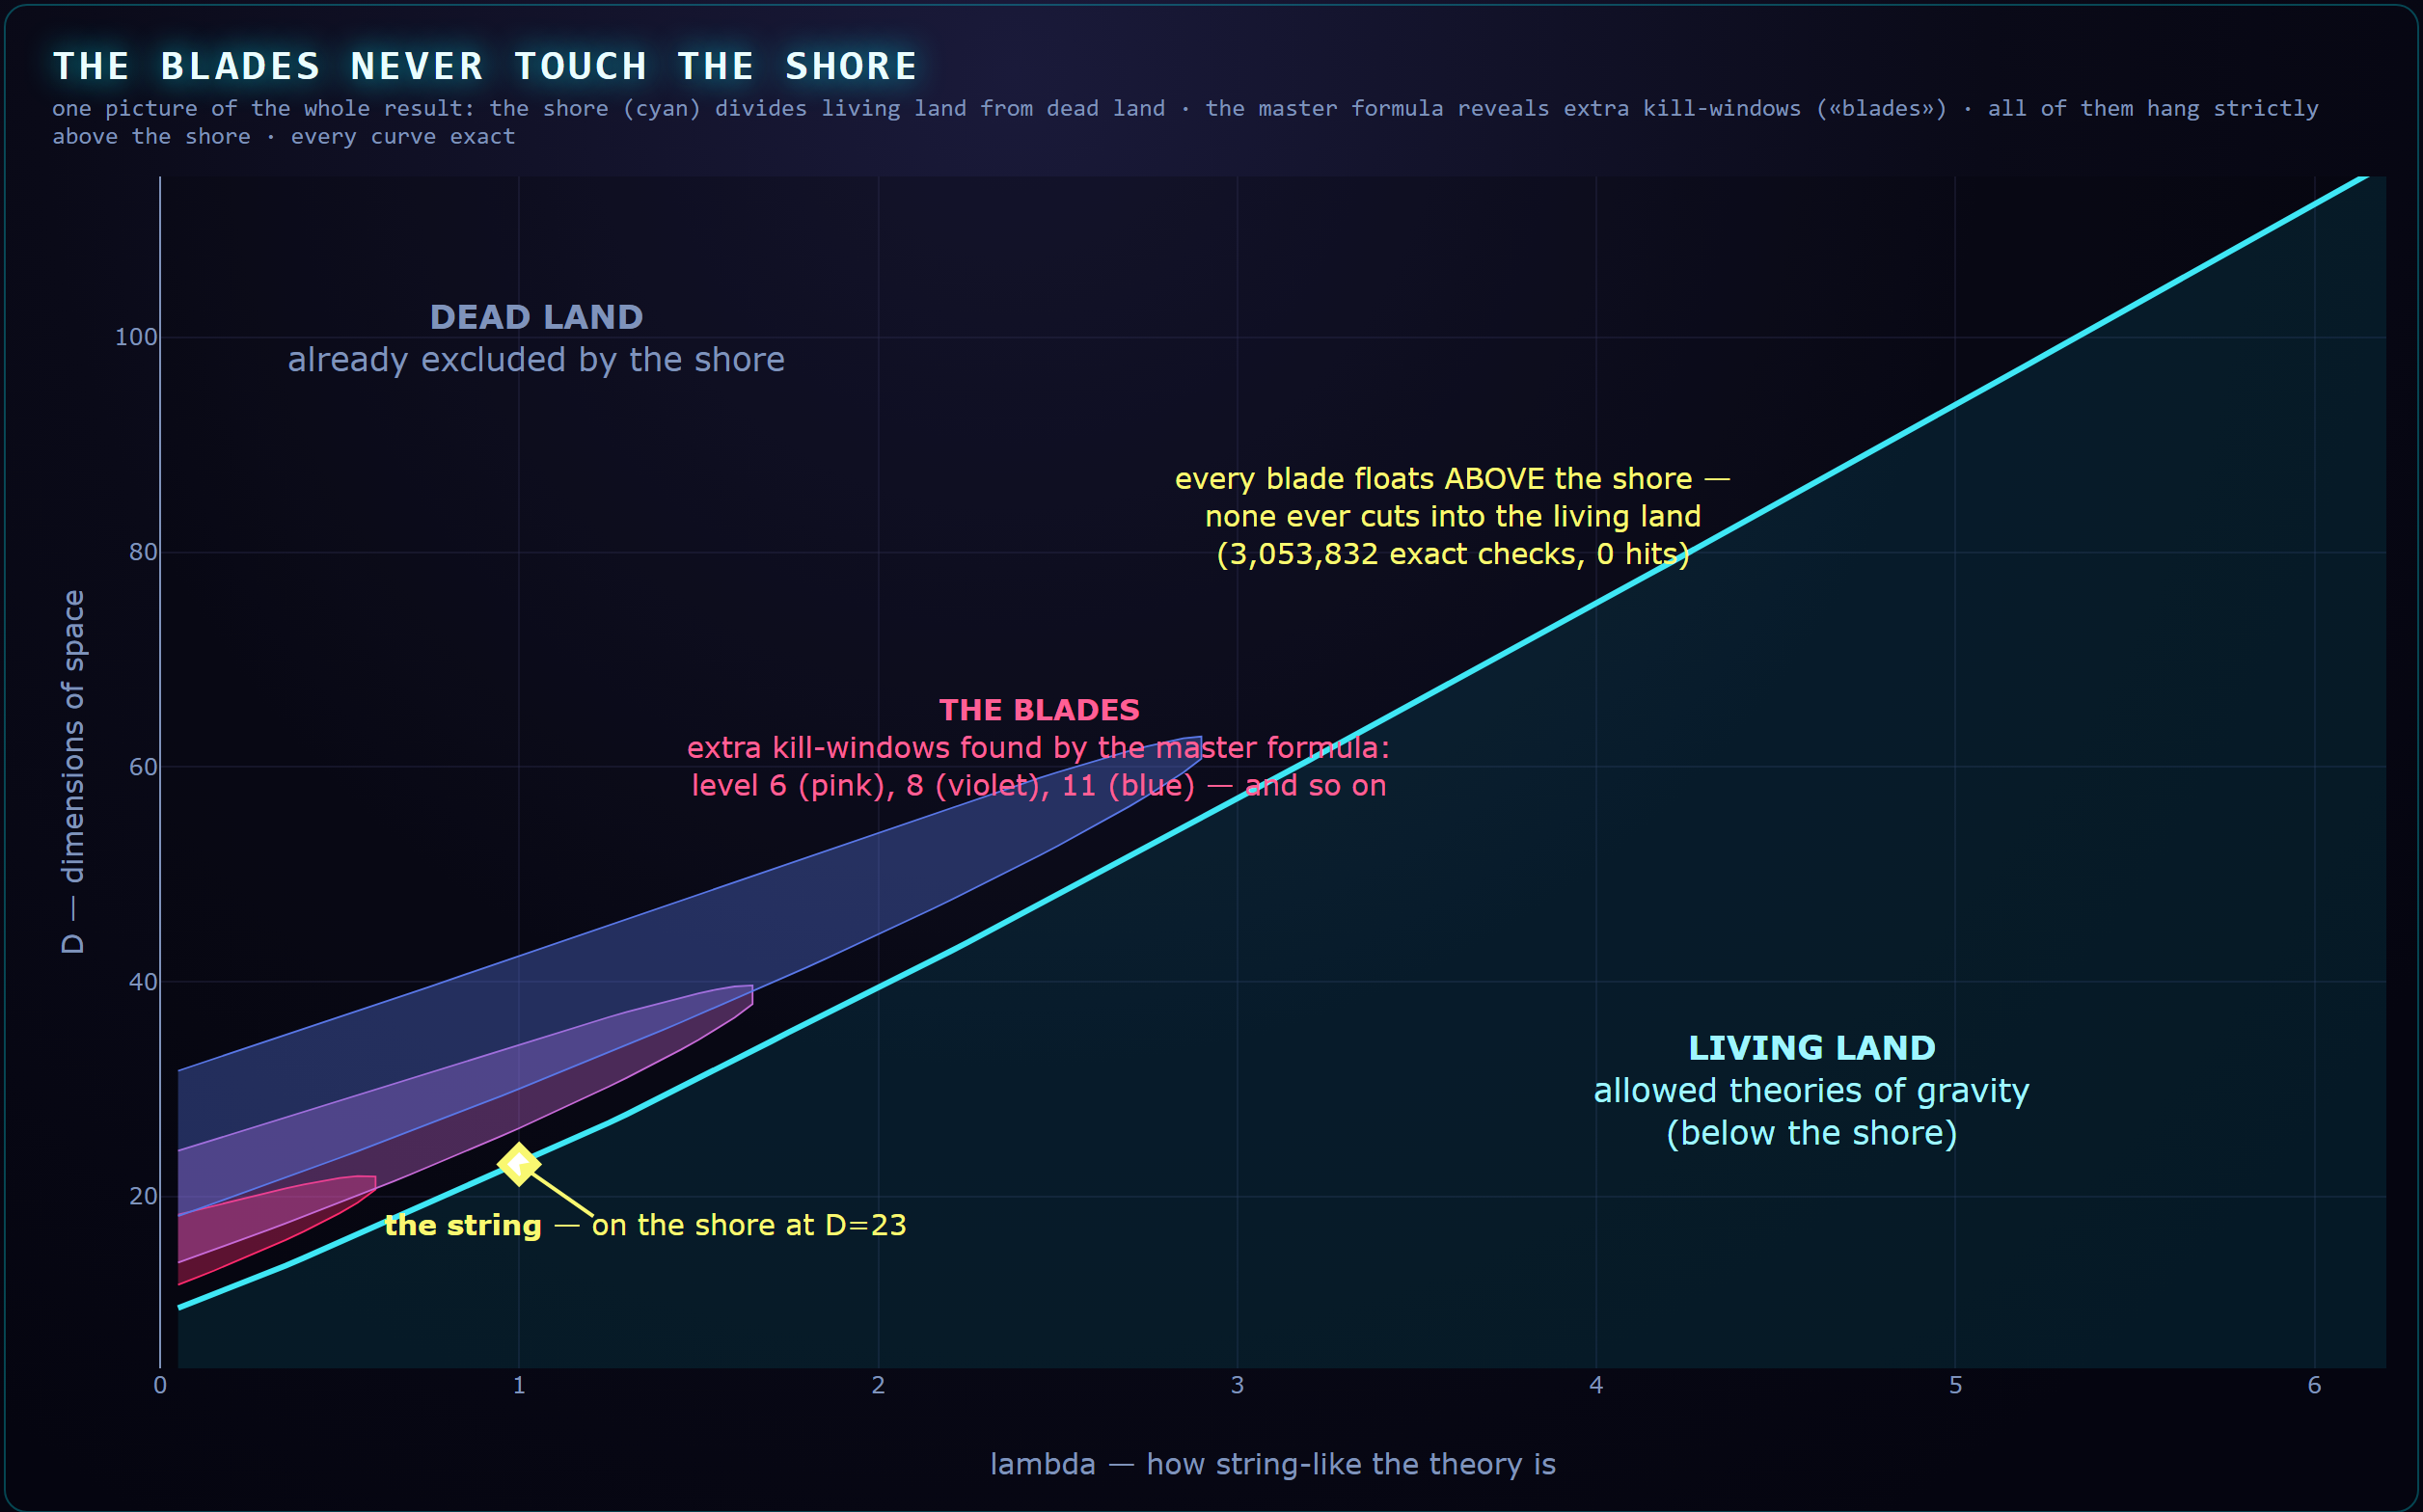
\includegraphics[width=\textwidth]{fig_knives.png}
\caption{The theorem, drawn. Blades: negativity windows of the second knife
(levels $6,8,11$), every curve exact; cyan: the shore; diamond: the string
at $D=23$. This paper proves no blade of any level, at any $\lambda$, ever
reaches the shore --- closest approach $2.17$ dimensions.}
\label{fig:knives}
\end{figure}

\section{Verification}
Beyond the certificates themselves (each is a finite list of nonnegative
rationals, re-checkable by inspection), the theorem was stress-tested:
$60{,}000$ random points across all regimes --- shallow water, deep water to
$\lambda=1500$, levels to $n=5000$, and the tangency direction --- found
minimum margin $2.18$ dimensions and no counterexample; the deep scans of
\cite{master} ($3{,}053{,}832$ points) are all implied by and consistent
with the theorem. [ADVERSARIAL-REVIEW-PLACEHOLDER]

\section{Discussion}
The completeness conjecture of \cite{shore} asserted that the near-leading
envelope is the true boundary of the family. For the second knife this is
now a theorem; for the higher knives ($j\ge4$) the master formula
\cite{master} gives the same ladder structure, the same asymptotic cone, and
a $3$-million-point clean battery --- the natural next step is to lift the
present certificate architecture to general $j$, for which
Lemma~\ref{lem:L2}'s containment and the exact tangency appear to be the
only two facts that need generalizing. String uniqueness within this family
would then rest, at every trajectory order, on proofs rather than scans.

\section*{Explain it to anyone}
Picture the coastline from our earlier papers: the shore where theories of
gravity die. Above it float blades --- extra danger zones we discovered with
the master formula. We had checked three million points and none of the
blades ever touched the shore. But checking is not knowing. This paper is
the proof: no blade, of any size, anywhere along the infinite coast, ever
touches the water. The subtle part is beautiful: infinitely far out, the
fleet of blades sails \emph{exactly parallel} to the shore --- tangent, zero
angle between them --- and the proof works only because every actual blade
is confined strictly inside the fleet's wake. Closest any blade ever comes:
about two dimensions of clearance.

\section*{Reproducibility and AI disclosure}
The entire proof re-runs from a single script (\texttt{blade\_proof.py}):
several hundred certificates, each a polynomial with nonnegative
coefficients after an explicit change of variables, all in exact arithmetic.
This research was conducted by the author working with an AI research
assistant (Claude, Anthropic). Two earlier prover architectures failed
honestly (a symbolic-branch drift and a missing no-window case) and are
recorded in the public log; the final architecture was adversarially
reviewed. [DISCLOSURE-REVIEW-PLACEHOLDER]

\begin{thebibliography}{9}
\bibitem{CHR2024b} C.~Cheung, A.~Hillman and G.~N.~Remmen,
``Uniqueness Criteria for the Virasoro-Shapiro Amplitude,''
Phys.\ Rev.\ D 111, 086034 (2025), arXiv:2408.03362.
\bibitem{shore} A.~Pluzhnik, ``The Shore of Closed-String Gravity,''
DOI 10.5281/zenodo.21944818.
\bibitem{master} A.~Pluzhnik, ``A Master Positivity Formula for the
Cheung--Hillman--Remmen Graviton Family,'' DOI 10.5281/zenodo.21947272.
\end{thebibliography}
\end{document}
